\subsection{Stopped Proton}

When we indicate the validity of charge response in high dE/dx region, proton is good sample due to its simple event structure.
At the same time, we verificate the recombination factor by proton in this analysis because proton has wide dE/dx range, and this is meaningless if the charge response of MC doesn't agree with that of DATA.
Therefore proton is very impotant in terms of comprehension of charge response.\\

First, protons are selected by the information of beam counters.
Then, proton events are applied following simple selections.\\

\begin{enumerate}
\item The drift time of the hit of the minimum channel number in the cluster is between 150$\mu$s$\sim$300$\mu$s(this time window is signal region). \\
\item The minimum channel number of hits in the cluster is below 2. \\
\item The maximum channel number of hits in the cluster is below 60. \\
\item The total hit number in the cluster is 5 or more. \\
\item The number of hits which are in the same channel is only one. \\
\end{enumerate}

We define the events which the number of clusters in the event which passed above selections is only one as good proton events.
For good proton events, we compare each paremeters of DATA and MC.
Figure\ref{fig:various_distribution} shows the comparison of the distribution of Hit Charge, Hit Sigma, Stopped Channel and  Cluster Charge between DATA and MC.
Table\ref{tb:various_distribution_comparison} shows the comparison of the mean of these distribution.

\begin{table}
  \centering
  \begin{tabular}[htb]{ccccccc}\hline
                        & DATA             & MC              & DATA/MC ratio       \\ \hline
    Hit Charge          & 607.5$\pm$19.6   & 622.3$\pm$0.8   & 0.9762$\pm$0.0316   \\
    Hit Sigma($\mu$s)   & 3.838$\pm$0.003  & 3.881$\pm$0.002 & 0.9889$\pm$0.0009   \\
    Stopped Channel     & 18.16$\pm$0.20   & 17.72$\pm$0.11  & 1.0247$\pm$0.0132   \\
    Cluster Charge      & 9940$\pm$407     & 9735$\pm$59     & 1.0210$\pm$0.0422   \\ \hline
  \end{tabular}
  \label{tb:various_distribution_comparison}
  \caption{Comparison of the mean of four distributions between DATA and MC}
\end{table}

All four distribution of MC reproduce DATA well.
Especially, the agreement of stopped channel distribution indicates the success of the momentum estimation by TOF infomation because where proton stopped depends on the initial momentum.\\

\begin{figure}[htbp]
  \centering
  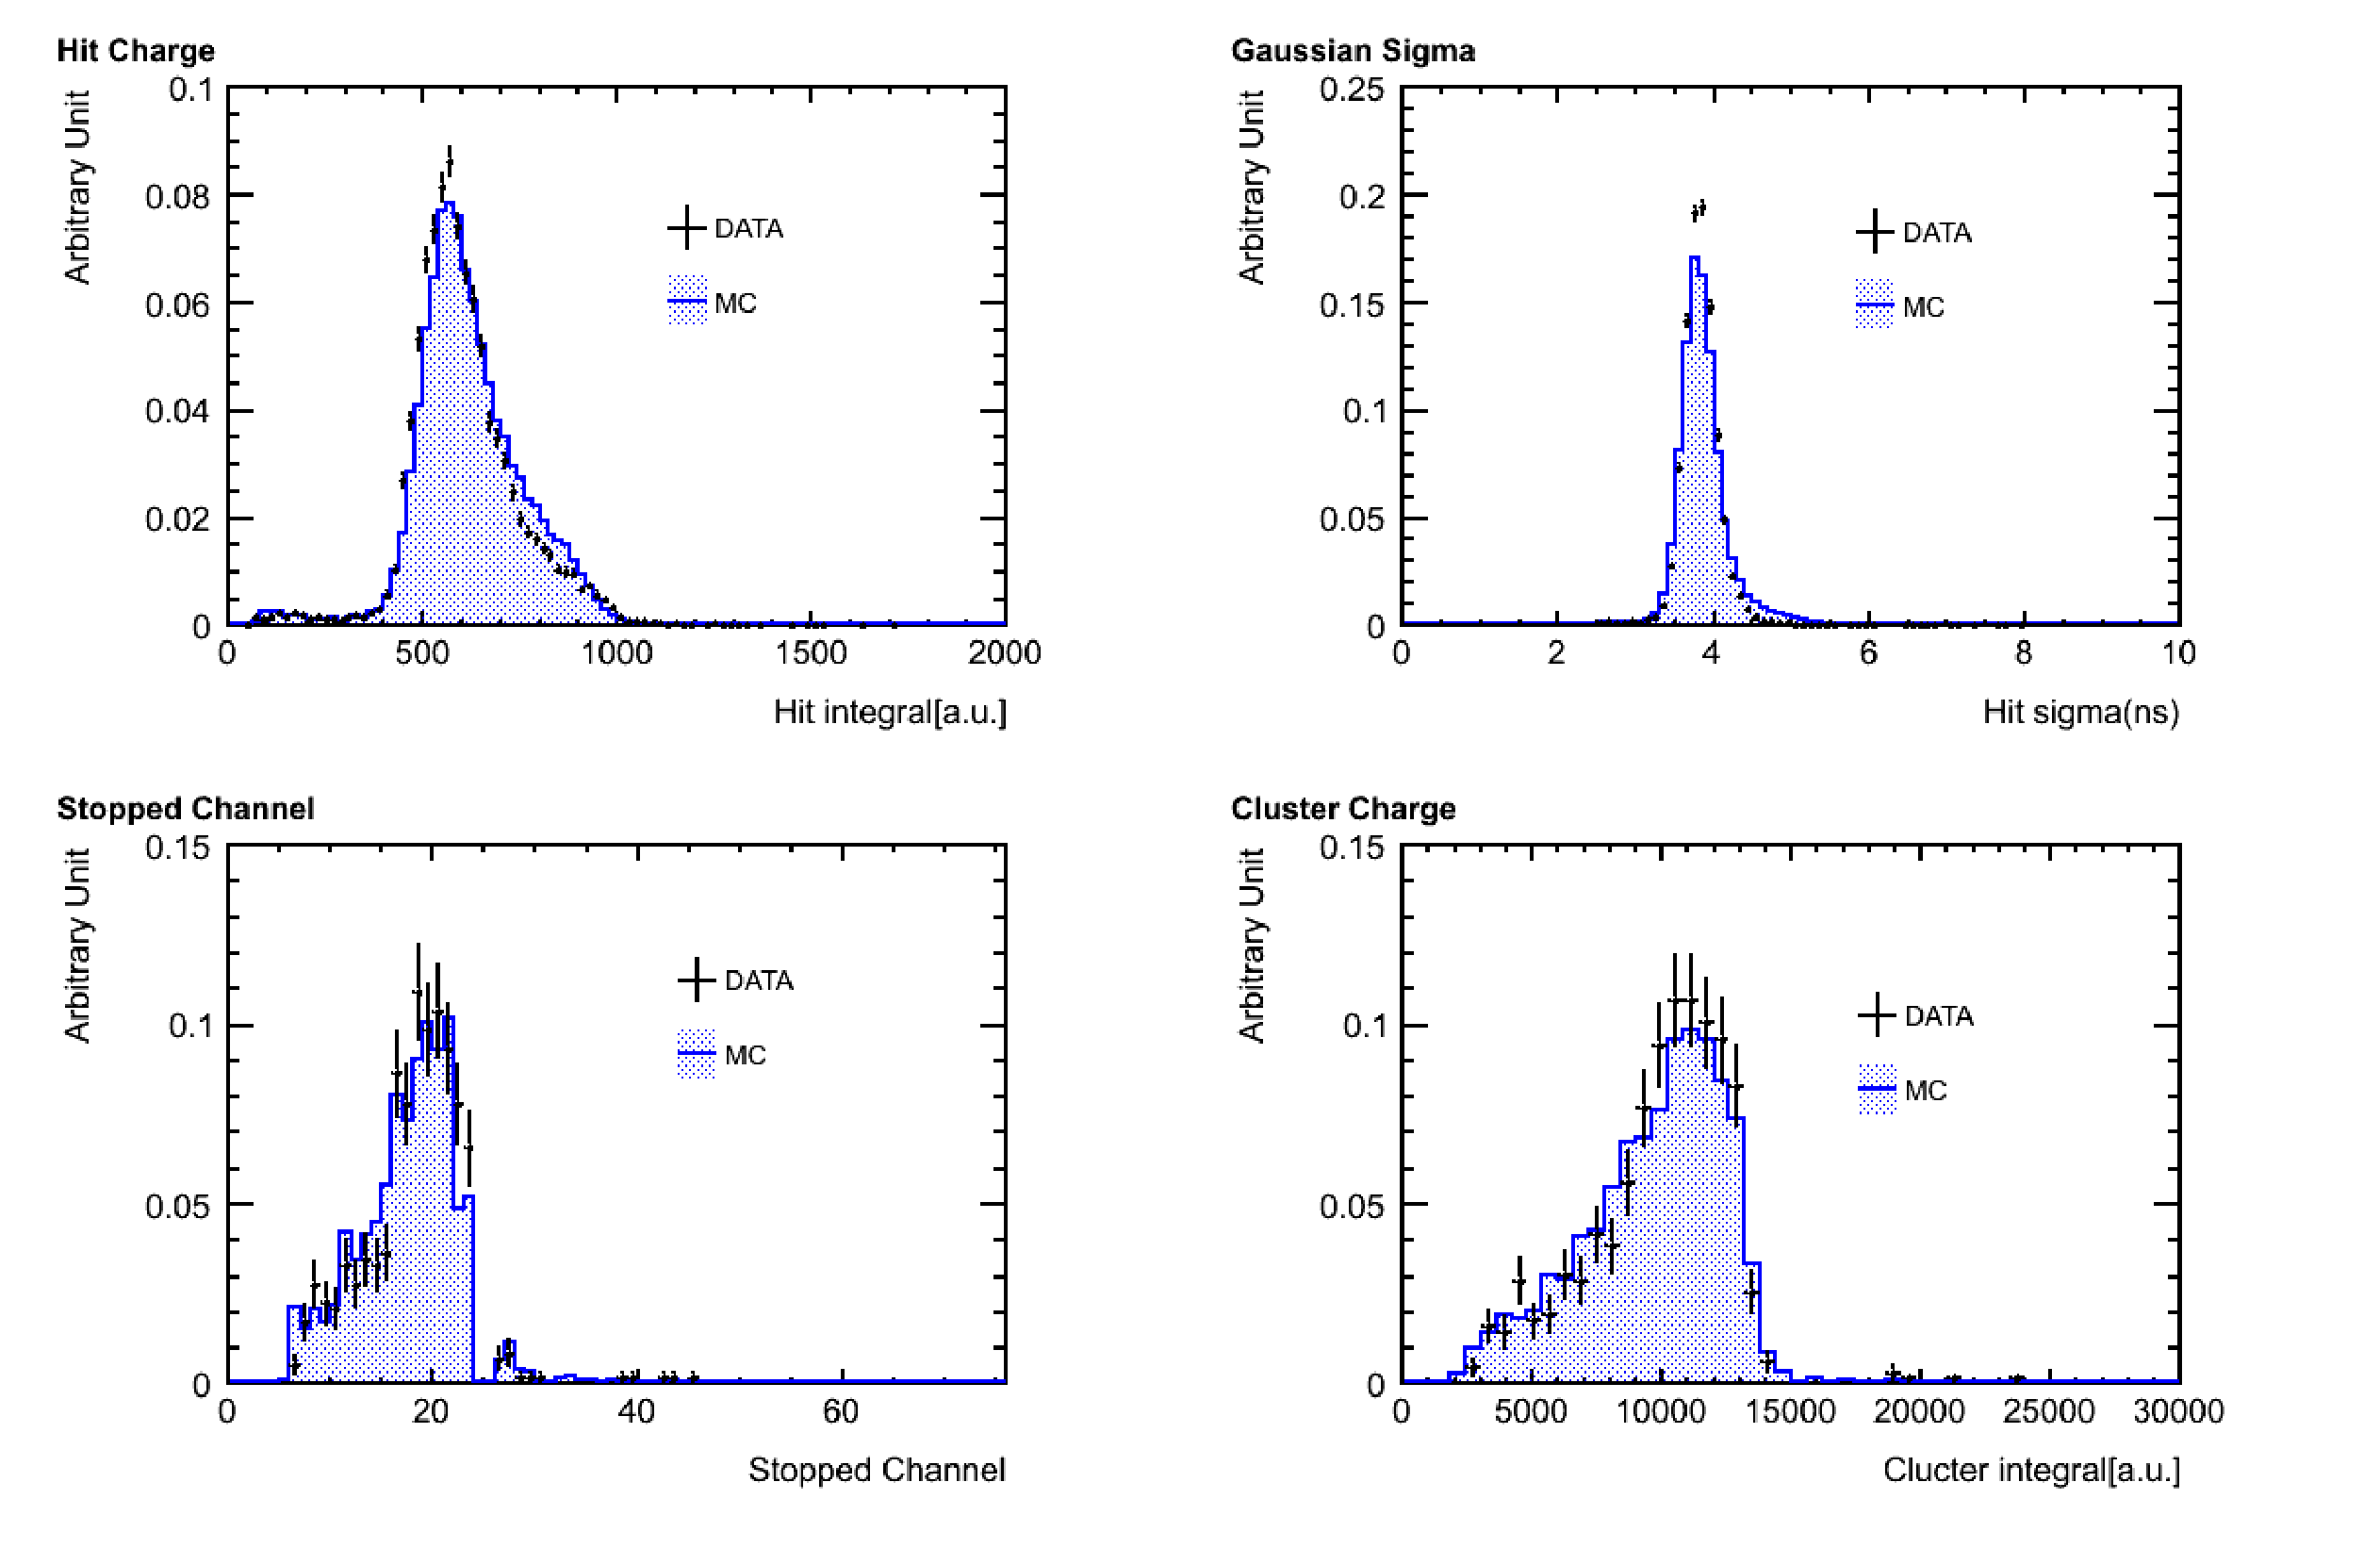
\includegraphics[width=10cm,clip]{./fig/stop_proton1.eps}
  \caption{DATA-MC comparison of Hit Charge, Hit Sigma, Stopped Channel, Cluster Charge}
  \label{fig:varios_distribution}
\end{figure}

Figure\ref{fig:ADC_distribution} shows the integrated ADC distribution of each channel from stopped channel.
The MC distribution of the channels after stopped channel are good agereements with DATA.\\
The left of figure\ref{fig:Mean_comparison} shows the mean of the above distribution of each channel.
The right of figure\ref{fig:Mean_comparison} shows the ratios of DATA/MC.
The ratios are surpressed within 94\%$\sim$105\%.
From this result, we succeed in reproducing the charge response of DATA in high and wide dE/dx region.

\begin{figure}[htbp]
  \centering
  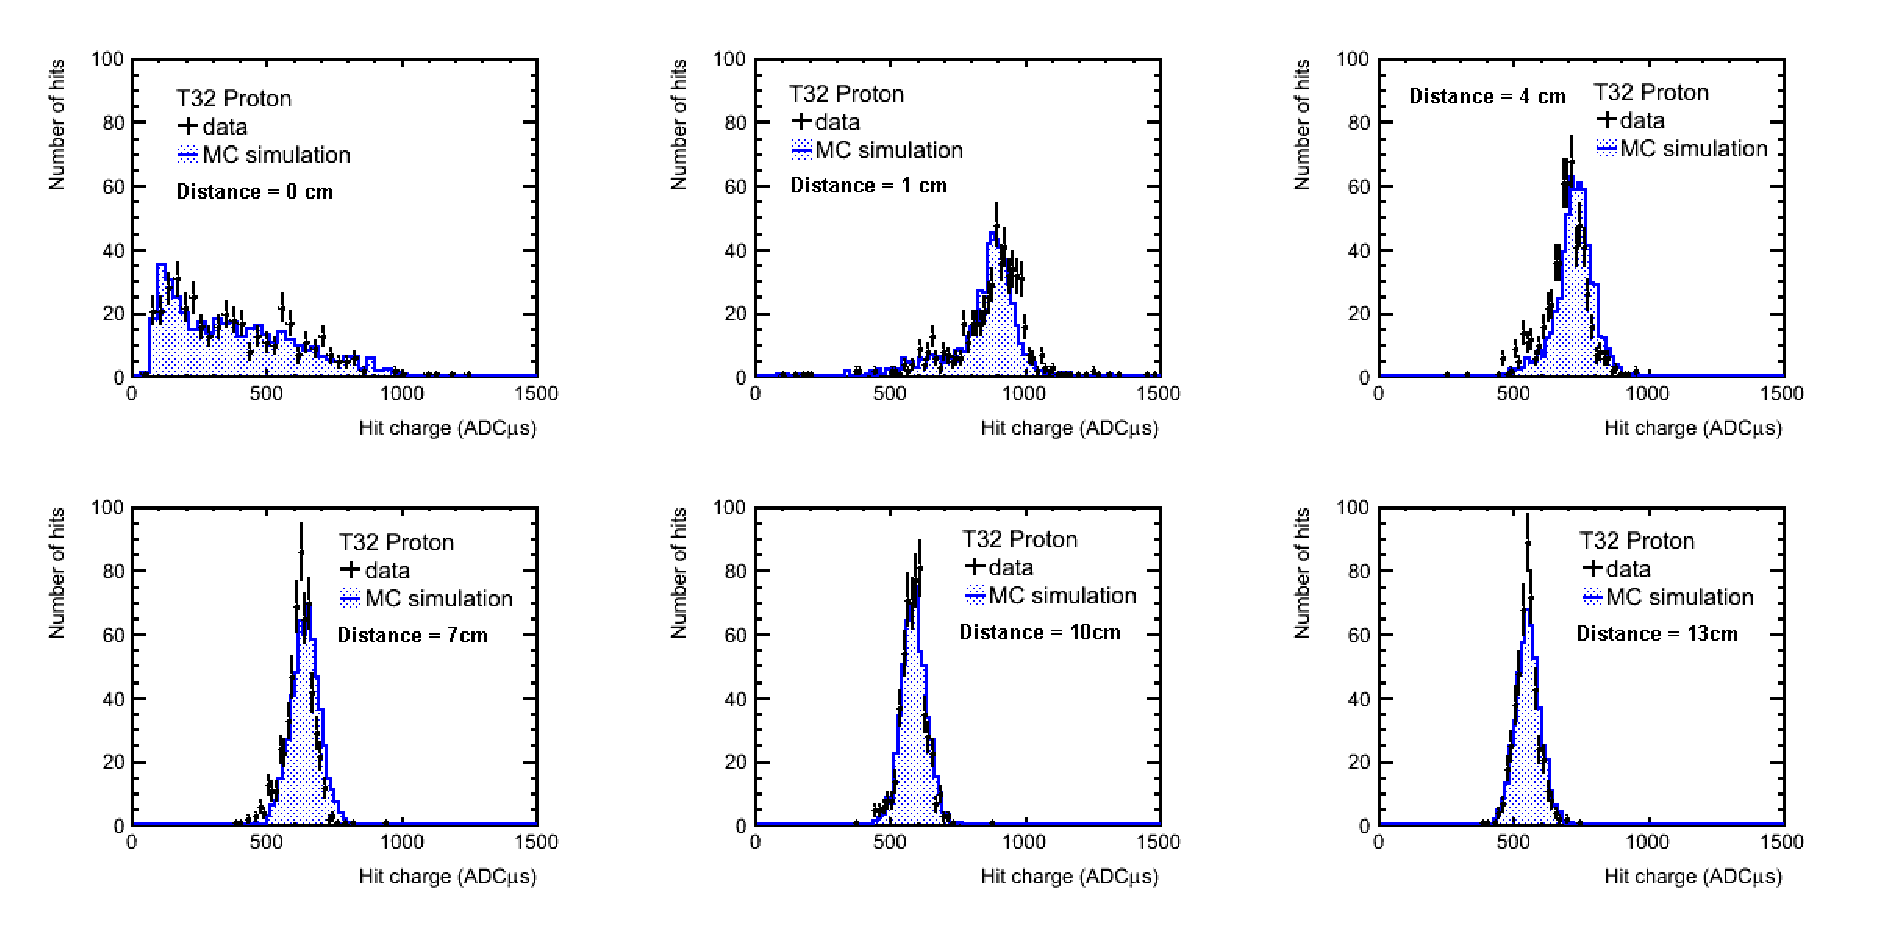
\includegraphics[width=10cm,clip]{fig/stop_proton2.eps}
  \caption{Integrared ADC distribution of each channel from stopped channel}
  \label{fig:ADC_distribution}
\end{figure}

\begin{figure}[htbp]
  \centering
  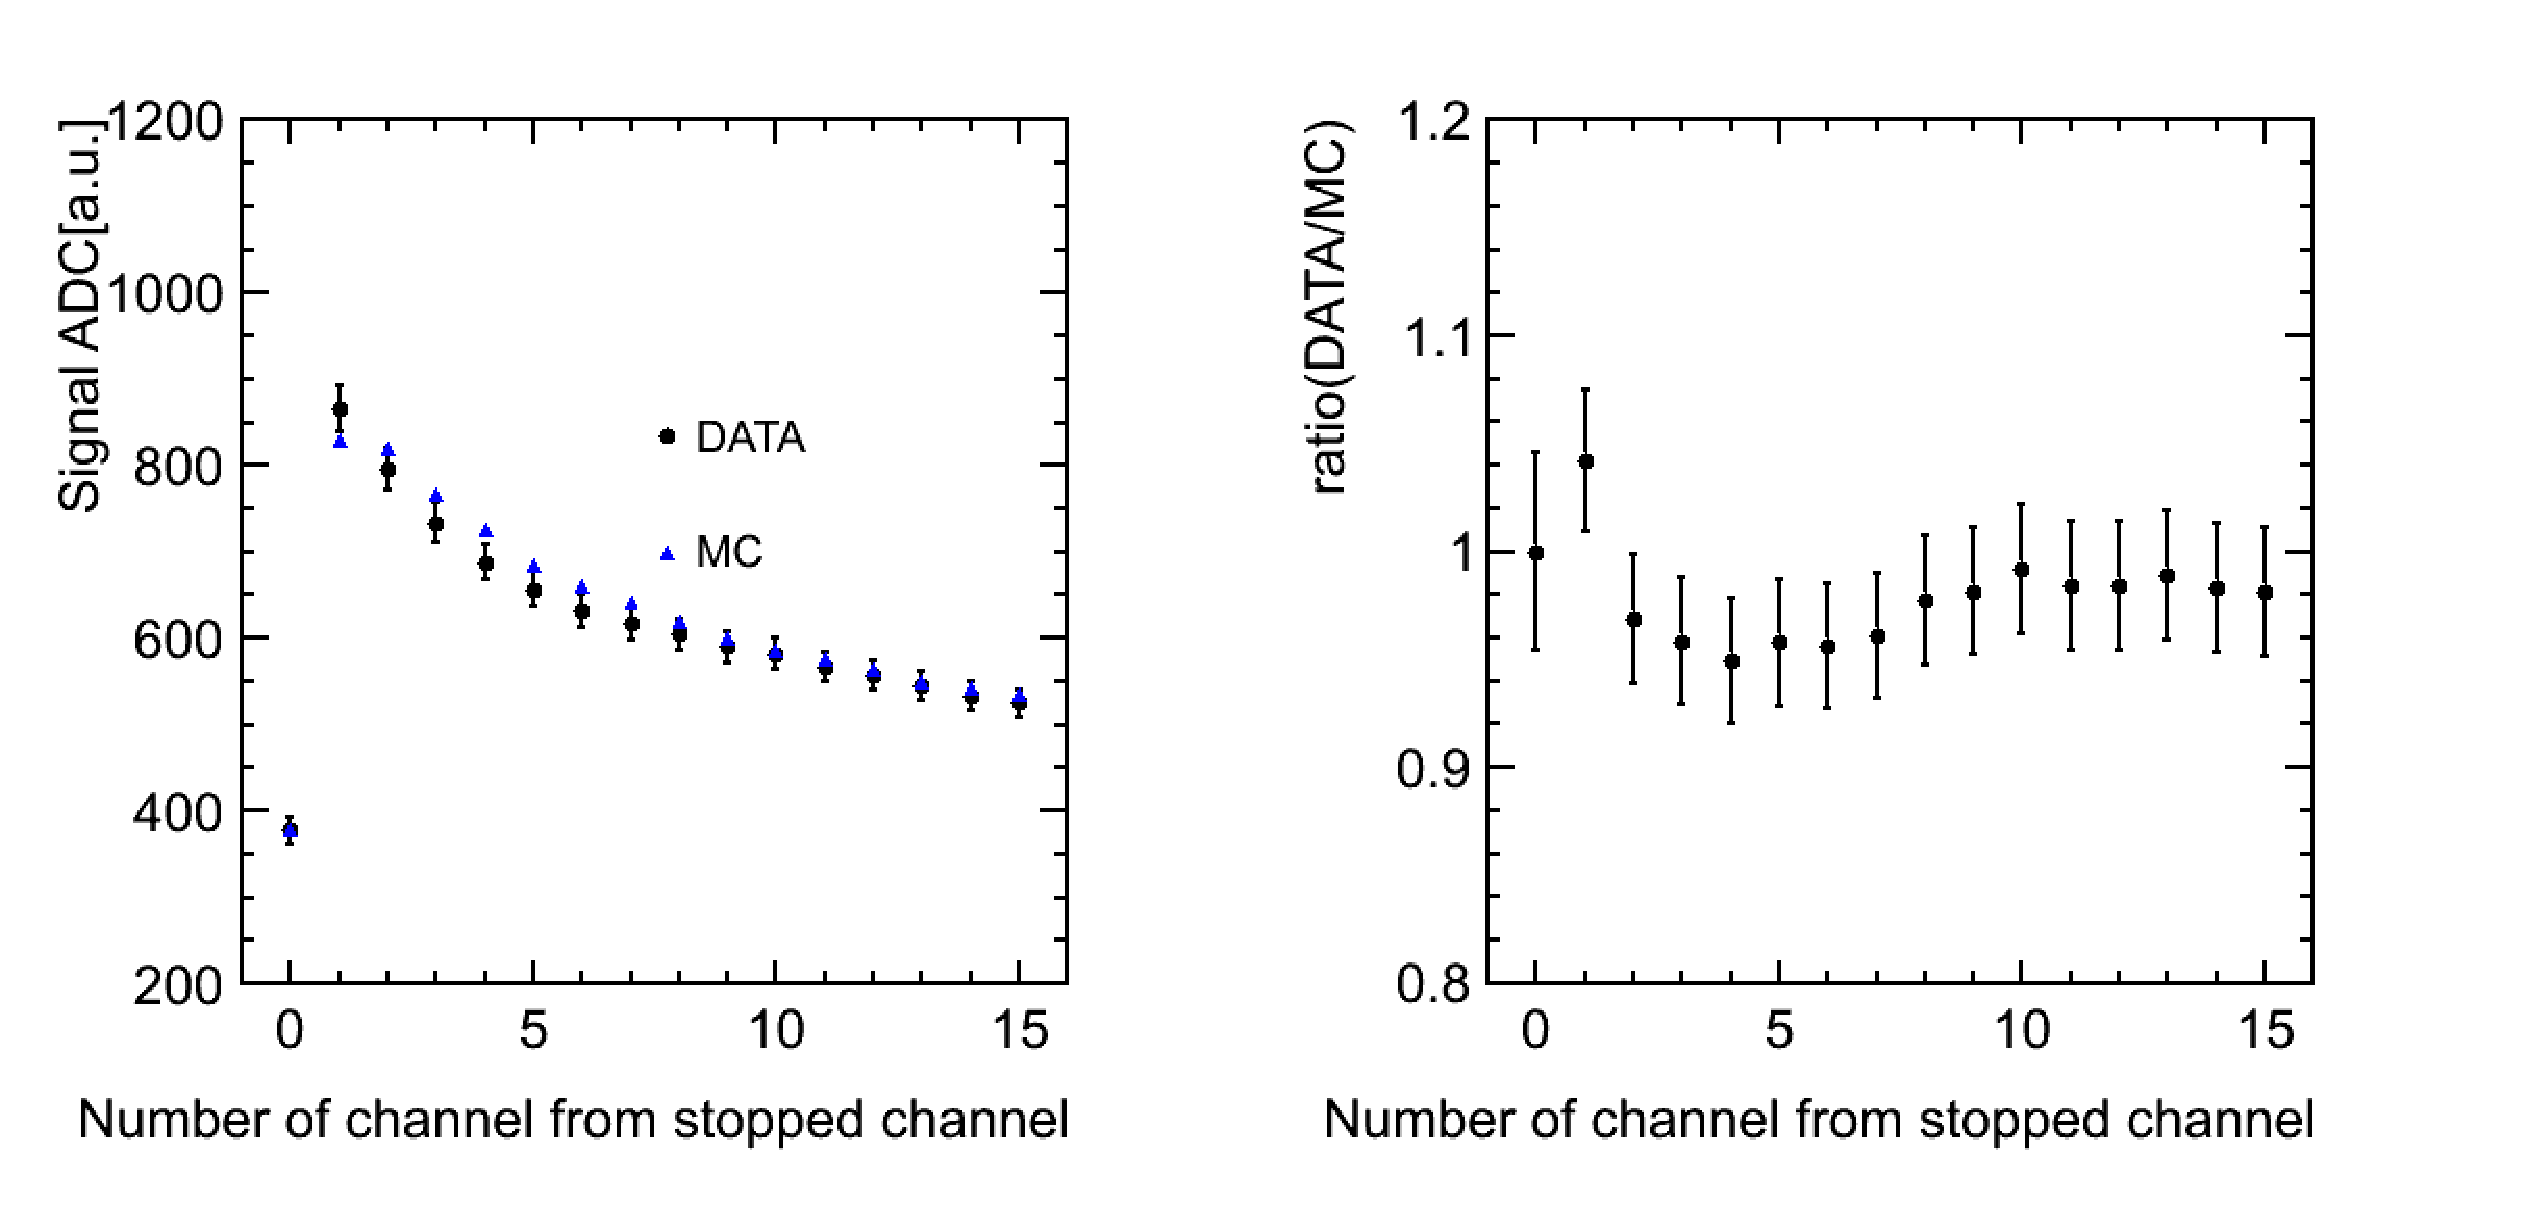
\includegraphics[width=10cm,clip]{fig/stop_proton3.eps}
  \caption{DATA-MC comparison of the mean of Integrated ADC distribution}
  \label{fig:Mean_comparison}
\end{figure}
